\itemhead{复习题三 · 第19题（教材p.92）}{XJ-B1-C03-RV-P092-Y1067}
\label{XJ-B1-C03-RV-P092-Y1067}
{\footnotesize 湘教版教材p.92 / PDF第99页 / 复习题三 / 第19题}
\field{原题}{探索并回答下列问题：
\subq{1}把 $y=\dfrac1x$ 的图象向右平移 1 个单位长度，求所得图象的函数解析式；
\subq{2}把 $y=\dfrac1x$ 的图象向左平移 2 个单位长度，求所得图象的函数解析式；
\subq{3}把 $y=\dfrac1x$ 的图象向上平移 1 个单位长度，求所得图象的函数解析式；
\subq{4}把 $y=\dfrac1x$ 的图象向下平移 2 个单位长度，求所得图象的函数解析式。
对于任意函数 $y=f(x)$，你能写出它的图象平移与解析式的变化规律吗？试一试。}
\field{参考答案}{依次为 $1/(x-1)$（$x\ne1$）、$1/(x+2)$（$x\ne-2$）、$1/x+1$、$1/x-2$（后二式 $x\ne0$）。一般向右平移 $h$ 用 $f(x-h)$，向上平移 $k$ 用 $f(x)+k$；定义域也随水平平移改变。}
\begin{center}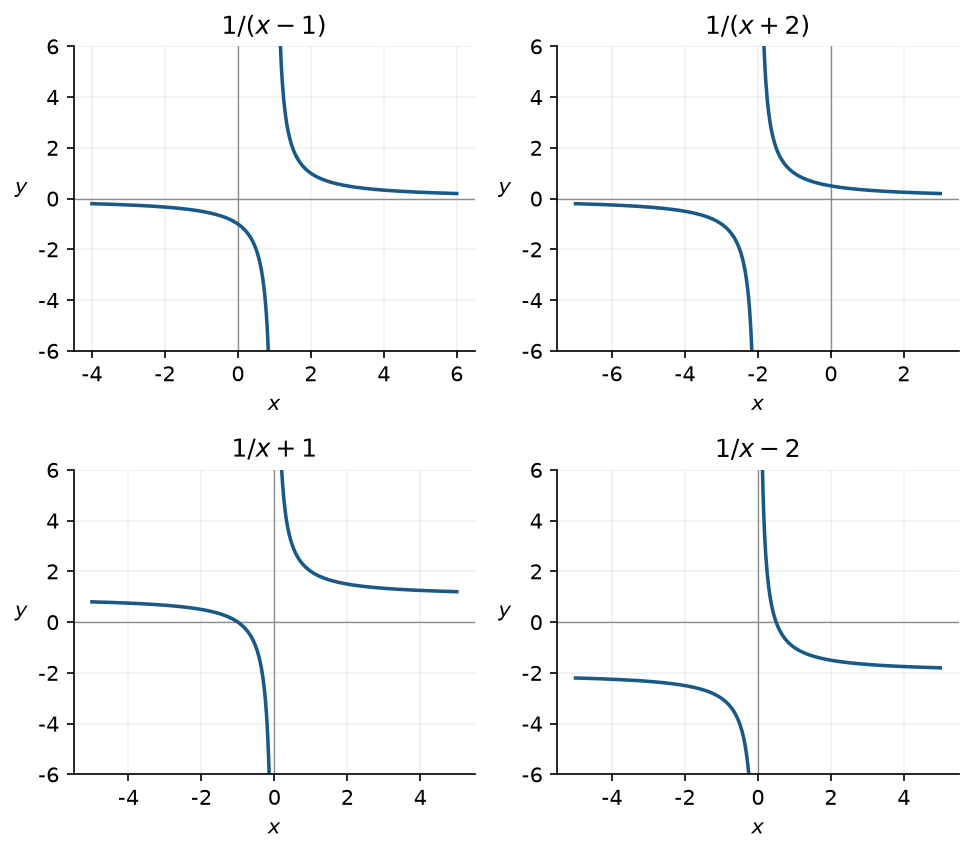
\includegraphics[width=.84\linewidth,height=.38\textheight,keepaspectratio]{figures/C03-RV092-19.png}\end{center}
{\small \field{关联知识}{F09 图象平移、伸缩与对称（教材帮p.86、94 / PDF95、103）；F02 定义域与原式限制（教材帮p.79、80、81 / PDF88、89、90）}
\field{方法与易错点}{追踪点 $(u,f(u))$ 变换后的坐标，反推新解析式。 易错：平移只改公式而未改定义域；把纵向倍率当作指数底数变化。}
\field{答案依据}{答案册相关题组：PDF第24、25、26、27页（册内页23、24、25、26）；按当前题库原题逐项重算，不按旧版题号机械对套。}}
